%\subsection{Histogramm f\"ur Property Instance (126)}
%\begin{figure}
\begin{center}
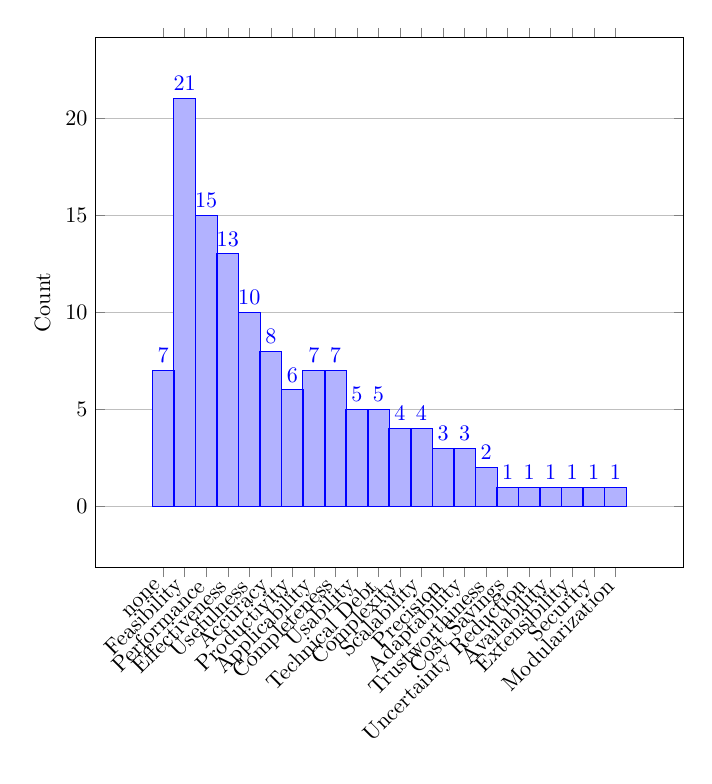
\begin{tikzpicture}[scale=.8]
\begin{axis}[ ybar, ymajorgrids, enlargelimits=0.15, legend style={at={(0.5,-0.15)}, anchor=north,legend columns=-1},
    width=.90\linewidth,height=10cm,
    nodes near coords, %nodes near coords align=below,
    ylabel={Count}, ymin=0,
    x tick label style={rotate=45,anchor=east},
    xtick={1,2,3,4,5,6,7,8,9,10,11,12,13,14,15,16,17,18,19,20,21,22},
    xticklabels={ none, Feasibility, Performance, Effectiveness, Usefulness, Accuracy,  Productivity, Applicability, Completeness, Usability, Technical Debt, Complexity, Scalability, Precision, Adaptability, Trustworthiness, Cost Savings, Uncertainty Reduction, Availability, Extensibility, Security, Modularization
}
    %xlabel={Property Instance}    
    ]
  \addplot coordinates { (1,7)  (2,21)  (3,15)  (4,13)  (5,10)  (6,8)  (7,6)  (8,7)  (9,7)  (10,5)  (11,5)  (12,4)  (13,4)  (14,3)  (15,3)  (16,2)  (17,1)  (18,1)  (19,1)  (20,1)  (21,1)  (22,1)   };
\end{axis}
\end{tikzpicture}
\end{center}
%\caption{Histogramm f\"ur Property Instance (126)}
%\label{fig:histo_propertyinstance}
%\end{figure}

